\documentclass{beamer}
\usepackage[T1]{fontenc}
\usepackage[utf8]{inputenc}
\usepackage{lmodern}
\usepackage[ngerman]{babel}

\usepackage{graphics}

\usepackage{amsmath}
\usepackage{booktabs}

\usepackage{dot2texi}
\usepackage{tikz}
\usetikzlibrary{arrows,shapes}
\usetikzlibrary{automata}

\usetheme{Singapore}
\usecolortheme{dove}
\graphicspath{{images/}{../comics/}}

\newcommand{\hiddencell}[2]{\action<#1->{#2}}

\AtBeginSection[]
{
  \begin{frame}[plain]
    \frametitle{}
    {\footnotesize
      \tableofcontents[currentsection]
    }
  \end{frame}
}

\title{Grundbegriffe der Informatik}
\author{Patrick Niklaus}

\begin{document}
\begin{frame}
  \frametitle{Grundbegriffe der Informatik}
  \framesubtitle{4. Tutorium}
  \begin{description}
    \item \textbf{Name:} Patrick Niklaus
    \item \textbf{E-Mail:} patrick.niklaus@student.kit.edu
    \item \textbf{Nr:} 43
  \end{description}
\end{frame}

\section{Übungsblatt}
\begin{frame}
  \frametitle{Anmerkungen zum letzten Übungsblatt}
  \begin{itemize}
    \item $k_{i+1} \longleftarrow k_i + 1$
    \item Schleifenkopf-Bedingung bei Vollständigen Induktion beachten.
    \item Immer hinschreiben aus welcher Menge eine Variable ist.
  \end{itemize}
\end{frame}

\section{Speicher}
\subsection{Bit}
\begin{frame}
	\frametitle{Bit}
	\begin{description}
		\item[Was ist ein Bit?] \only<2->{Ein Zeichen aus dem Alphabet $\{0,1\}$}
	\end{description}
	\pause
	\pause
	\begin{block}{Herkunft des Namens}
		\begin{itemize}
			\item \textbf{bi}nary dig\textbf{it}
			\item \textbf{B}asic Indissoluble \textbf{I}nformation Uni\textbf{t}
		\end{itemize}
	\end{block}
	\pause
	\begin{block}{Abkürzung}
		$b$ oder $bit$
	\end{block}
\end{frame}

\subsection{Byte}
\begin{frame}
	\frametitle{Byte}
	\begin{description}
		\item[Was ist ein Byte?] Ein Wort über dem Alphabet $\{0,1\}$ der Länge 8\footnote{ursprünglich der Länge 6}
	\end{description}
	\pause
	\begin{block}{Herkunft des Namens}
		In Anlehnung an die englischen Wörter \textit{bit} und \textit{bite}.\\
		Oft auch als \textit{Octet} bezeichnet.
	\end{block}
	\pause
	\begin{block}{Abkürzung}
		$B$ für $Byte$\\
		$o$ für $Octet$\\
	\end{block}
\end{frame}

\subsection{Größenpräfixe}
\begin{frame}[plain]
	\frametitle{Speicher-Präfixe}
	Um die Größe von "`großen"' Speichern zu beschreiben verwendet man Präfixe:
	\begin{block}{Dezimal}
		\begin{tabular}{rccc}
			1000&$10^{3}$&kilo&k\\
			1000000&$10^{6}$&mega&M\\
			1000000000&$10^{9}$&giga&G\\
			1000000000000&$10^{12}$&tera&T\\
			1000000000000000&$10^{15}$&peta&P\\
			1000000000000000000&$10^{18}$&exa&E\\
		\end{tabular}

	\end{block}
	\begin{block}{Binär}
		\begin{tabular}{rccc}
			$1024$&$2^{10}$&kibi&ki\\
			$1048576$&$2^{20}$&mebi&Mi\\
			$1073741824$&$2^{30}$&gibi&Gi\\
			$1,099511628*10^{12}$&$2^{40}$&tebi&Ti\\
			$1,125899907*10^{15}$&$2^{50}$&pebi&Pi\\
			$1,152921505*10^{18}$&$2^{60}$&exbi&Ei\\
		\end{tabular}
	\end{block}

\end{frame}


\subsection{Speicher als Abbildung}
\begin{frame}
	\frametitle{Speicher als Abbildung}
	\begin{tabular}{cc}
		\toprule
		Adresse&Wert\\
		\midrule
		000&10101000\\
		001&01101001\\
		010&01010011\\
		011&10100110\\
		100&11001101\\
		101&11011001\\
		110&00101011\\
		111&00000100\\
		\bottomrule
	\end{tabular}
	\begin{block}{Relation}
		$m:\text{Adr}\rightarrow\text{Val}$\\
		\vspace{.2cm}
		Der an der Stelle $a\in$ Adr gespeicherte Wert $v\in$ Val ist $m(a)$.
	\end{block}
\end{frame}

\begin{frame}
	\frametitle{Speicher als Abbildung}
	\begin{exampleblock}{Beispiel}
		Gegeben sei ein Rechner mit 8\,GiB Hauptspeicher. Mit einer Adresse adressiert man ein Byte.\\
		Wie sieht die Abbildung $m$ für diesen Fall aus?
		\pause
		\begin{equation*}
			m:\{0,1\}^{64}\rightarrow \{0,1\}^8
		\end{equation*}
	\end{exampleblock}
\end{frame}




\section{Von Wörtern zu Zahlen und zurück}
\subsection{Dezimaldarstellung von Zahlen}
\begin{frame}
	\frametitle{Dezimaldarstellung von Zahlen}
	\begin{definition}
		Gegeben sei ein Alphabet $Z_{10}=\{0,1,2,3,4,5,6,7,8,9\}$\\
		\vspace{.5cm}
		$\forall x\in Z_{10}:\text{num}_{10}(x)$ ist der Zahlenwert von $x$.
		\pause
		\begin{eqnarray*}
			\text{Num}_{10}(\varepsilon)&=&0\\
			\forall w\in Z_{10}^* \forall x\in Z_{10}: \text{Num}_{10}(wx)&=&10\cdot \text{Num}_{10}(w)+\text{num}_{10}(x)
		\end{eqnarray*}
	\end{definition}
\end{frame}

\subsection{Andere Zahldarstellungen}
\begin{frame}
	\frametitle{Andere Zahldarstellungen}
	\begin{block}{Umwandlung}
		Num$_k(wx)=k\cdot$Num$_k(w)+$num$_k(w)$
	\end{block}
	\pause
	\begin{exampleblock}{Beispiel}
		\begin{itemize}
			\item Num$_2(101010)=\only<3->{42}$
			\item Num$_3(1021)=\only<4->{34}$
			\item \only<-8>{Num$_2(1)=\only<5->{1}$}\only<9->{Num$_3(2)=\only<10->{2}$}
			\item \only<-8>{Num$_2(11)=\only<6->{3}$}\only<9->{Num$_3(22)=\only<11->{8}$}
			\item \only<-8>{Num$_2(111)=\only<7->{7}$}\only<9->{Num$_3(222)=\only<12->{26}$}
			\item \only<-8>{Num$_2(1111)=\only<8->{15}$}\only<9->{Num$_3(2222)=\only<13->{80}$}
		\end{itemize}

	\end{exampleblock}
\end{frame}

\begin{frame}
	\frametitle{Algorithmus zur Umwandlung Binärdarstellung $\rightarrow$ Zahl}
	// Eingabe: $w\in Z_2^*$\\
	x $\leftarrow$ 0\\
	\visible<4->{$v\leftarrow \varepsilon$\\}
	\visible<2->{\textbf{for} $i\leftarrow 0$ \textbf{to} $|w|-1$ \textbf{do}\\
	\visible<4->{\hspace{0.4cm}$v\leftarrow v\cdot w(i)$\\}
	\hspace{.4cm}$x\leftarrow 2x+$ num$_2(w(i))$\\
	\textbf{od}\\}

	// Hier soll gelten: \visible<3->{$x =$ Num$_2(w)$}
\end{frame}


\section{Übersetzungen}
\subsection{Warum?}
\begin{frame}
	\frametitle{Wozu Übersetzungen?}
	\pause
	\begin{itemize}
		\item Lesbarkeit
		\item Kompression
		\item Verschlüsselung
		\item Fehlererkennung und -korrektur
		\item \dots
	\end{itemize}
\end{frame}

\subsection{Homomorphismen}
\begin{frame}
	\begin{exampleblock}{Beispiel}
		$h(a)=001$\\
		$h(b)=1101$\\
		Also gilt:
		\begin{eqnarray*}
			h^{**}(bba)&=&h(b)h(b)h(a)\\
			&=&1101\cdot 1101\cdot 001\\
			&=&11011101001
		\end{eqnarray*}
	\end{exampleblock}
	\pause
	\begin{definition}
		Der Homomorphismus $h^{**}:A^*\rightarrow B^*$ sei wie folgt definiert:
		\begin{eqnarray*}
			h^{**}(\varepsilon)&=&\varepsilon \\
			\forall w\in A^*:\forall x\in A:h^{**}(wx)&=&h^{**}(w)h(x)
		\end{eqnarray*}
	\end{definition}
\end{frame}

\subsection{$\varepsilon$-freier Homomorphismus}
\begin{frame}
	\frametitle{$\varepsilon$-freier Homomorphismus}
	\begin{definition}
		Ein Homomorphismus ist $\varepsilon$-frei, wenn für alle $x\in A$ gilt: $h(x)\neq \varepsilon$.
	\end{definition}

	Warum sollte ein Homomorphismus $\varepsilon$-frei sein?
	\begin{exampleblock}{Beispiel}
		$h(a)=001$\\
		$h(b)=\varepsilon$\\
		\pause
		Es sei $h(w)=001$. Dann ist $w$ nicht eindeutig bestimmt.
		Es ist "`Information verloren gegangen"'.
	\end{exampleblock}
\end{frame}
\begin{frame}
	\frametitle{"`Informationsverlust"'}
	\begin{exampleblock}{Beispiel}
		$h(a)=0$\\
		$h(b)=1$\\
		$h(c)=10$\\
		\visible<2->{$h(bac)=1010$}\visible<3->{$=h(cba)=h(cc)$}
	\end{exampleblock}
	\begin{itemize}
		\item Warum geht bei dieser Übersetzung Information verloren?
		\pause
		\item Wie kann man allgemein ausdrücken, wann Information verloren geht?\\
		\visible<3->{$\exists w_1\neq w_2$ mit $h^{**}(w_1)=h^{**}(w_2)$}
	\end{itemize}
	\pause
\end{frame}
\subsection{Präfixfreiheit}
\begin{frame}
	\frametitle{Präfixfreiheit}
	\begin{definition}
		Für keine zwei Symbole $x_1,x_2\in A$ gilt: $h(x_1)$ ist Präfix von $h(x_2)$
	\end{definition}
	\begin{exampleblock}{Beispiele}
		Welche Codierungen sind präfixfrei?:
		\begin{itemize}
			\item $h(a)=001, h(b)=1101 $ \pause \checkmark\\
			\item $h(a)=01, h(b)=011 $ \pause x\\
			\item $h(a)=011, h(b)=110 $ \pause \checkmark\\
			\item $h(a)=42, h(b)=4, h(b)=24 $ \pause x\\
		\end{itemize}

		
	\end{exampleblock}

\end{frame}





\section{Huffman-Codierung}
\subsection{Aufgaben}
\begin{frame}
	\begin{block}{Aufgabe}
		Gegeben sei das Wort $eaebcaebacbde$.
		\begin{enumerate}
			\item Konstruiere den dazugehörigen Huffman-Baum
			\item Codiere das Wort
		\end{enumerate}
	\end{block}
\end{frame}

\begin{frame}
	\begin{block}{Aufgabe}
		\begin{itemize}
			\item Codiere das Wort $badcfehg$.
			\item Wie lang wird die Codierung?
		\end{itemize}
	\end{block}
	\begin{block}{Aufgabe}
		\begin{itemize}
			\item Es sei folgende Zeichenverteilung gegeben:
		\end{itemize}
			\begin{tabular}{ccccccccc}
				\toprule
				Zeichen&a&b&c&d&e&f&g&h\\
				\midrule
				Häufigkeit&1&2&4&8&16&32&64&128\\
				\bottomrule
			\end{tabular}
		\begin{itemize}
			\item Codiere erneut das Wort $badcfehg$.
			\item Wie lang wird dieses Mal die Codierung?
		\end{itemize}
	\end{block}
\end{frame}

\begin{frame}[plain]
	\begin{block}{Klausur-Aufgabe}
  Gegeben sei ein Wort uber dem Alphabet $A = \{a, b, c, d\}$ mit folgenden relativen Häufigkeiten:
    \begin{tabular}{ccccccccc}
      \toprule
      Zeichen&a&b&c&d&\\
      \midrule
      Häufigkeit & x & $\frac{1}{4}$ & $\frac{1}{4}$ & $\frac{1}{2} - x$\\
      \bottomrule
    \end{tabular}\\
    $0 \leq x \leq \frac{1}{4}$\pause
		\begin{enumerate}
			\item Konstruieren Sie den Huffman-Baum für $x = \frac{1}{16}$.
      \item Welche Struktur muss der Huffman-Baum haben, damit die Huffman-Codierung
            eines Wortes $w \in A^+$ mit den in der Tabelle angegebenen relativen
            Häufigkeiten echt kürzer als $2|w|$ sein kann?
      \item Für welche $x \in \mathbb{R}$ mit $0 \leq x \leq \frac{1}{4}$ werden Wörter
            mit den angegebenen relativen Häufigkeiten auf genau doppelt so
            lange Wörter über $\{0, 1\}$ abgebildet?
		\end{enumerate}
	\end{block}
\end{frame}


\section{Abschluss}
\subsection{Zusammenfassung}
\begin{frame}
  \frametitle{Was ihr jetzt wissen sollte.}
  \begin{enumerate}
    \item Was sind Bit/Bytes?
    \item Präfix-Unterschiede Basis 10 und Basis 2.
    \item Wie rechne ich von einem Zahlensystem in ein anderes um?
    \item Was ist ein Homomorphismus?
    \item Was heißt $\varepsilon$-frei?
    \item Was heißt prefixfrei?
    \item Wie konstruiere ich einen Huffman-Baum?
    \item Wie lese ich darauf ein Codewort ab?
  \end{enumerate}
\end{frame}

\subsection{xkcd}
\begin{frame}[plain]
  \begin{figure}
    \begin{center}
      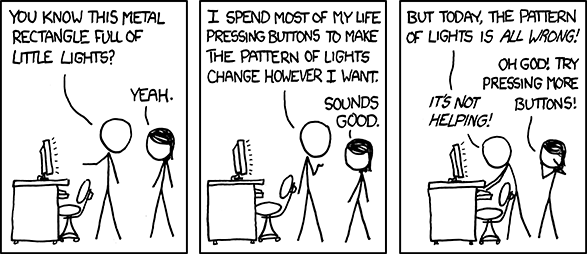
\includegraphics[width=320pt]{computer_problems}
    \end{center}
  \end{figure}
\end{frame}

\end{document}
